\chapter{Implementierung Device}
\label{cha:impl_device}

\section{Technologische Grundlagen}
\subsection{Android}
%TODO evtl. ein kurzer Abschnitt über Android, Java, die App auf der Brille?

\subsection{Visualisierung der Regale}
Für einige Prozesse auf der Brille ist es erforderlich, dass die exakte Position eines Produktes in einem Regal auf der Verkaufsfläche angezeigt wird. Dazu gibt es unter Verwendung von Wearable Computern grundsätzlich zwei Möglichkeiten:

\begin{enumerate}
	\item Das Regal wird abstrahiert und schematisch in einer vereinfachten Form dargestellt. Innerhalb dieser Darstellung wird die Position des gesuchten Produktes im Regal markiert. Der Benutzer muss selbst die Verknüpfung zwischen der Darstellung und der Realität herstellen, wenn er vor dem Regal steht.
	\item Durch Nutzung einer Videokamera wird die Umgebung des Benutzers und somit das Regal digital erfasst und durch Bild-im-Bild-Überlagerung die Produktposition im Regal markiert. Die Verknüpfung von Darstellung und Realität ist dadurch sehr stark. Voraussetzung ist hierbei jedoch, dass der Benutzer sich direkt vor dem Regal befindet -- andernfalls ist wiederum eine abstrahierte Darstellung erforderlich.
\end{enumerate}

Für die Umsetzung des Systems im Rahmen dieser Arbeit wurde die erste Möglichkeit gewählt, da sie technisch einfacher umzusetzen ist und zugleich auch eine Umsetzung der zweiten Möglichkeit vorbereitet.

Für die schematische Darstellung des Regals wurde die Ansicht gewählt, die ein Benutzer hat, wenn er sich vor dem Regal befindet (Frontalansicht oder Draufsicht). Regale sind rechteckig, ebenso wie Regalfächer, und lassen sich jeweils über Höhe und Breite, sowie bei den Fächern über die Position im Regal beschreiben. Dies sind optimale Voraussetzungen für die Umsetzung als zweidimensionale Ansicht.

Die technische Umsetzung der schematischen Darstellung kann i.A. auf drei Arten erfolgen:

\begin{enumerate}
	\item als Bitmap (pixelbasierte Grafik);
	\item als Vektorgrafik, also eine mathematisch beschriebene Grafik, die bei Ausgabe auf Bildschirmen verlustfrei in eine Bitmap der gewünschten Auflösung umgewandelt wird; oder
	\item als \acs{3D}-Grafik, die zusätzlich noch Tiefeninformationen speichert.
\end{enumerate}

Für die Darstellung auf dem Gerät fiel die Entscheidung auf eine Umsetzung als Vektorgrafik im \acs{SVG}-Format. Eine \acs{SVG}-Grafik ist im Grunde eine \acs{XML}-Datei, besteht also aus Text. Grundformen wie Rechtecke lassen sich über \acs{SVG} sehr einfach beschreiben, und für die Darstellung eines Regals werden keine komplizierteren Formen benötigt. Dies ist sehr platzsparend im Vergleich zu Bitmaps mit dem selben visuellen Inhalt. Außerdem können im \acs{XML}-Code der \acs{SVG}-Grafik weitere Informationen über das Regal und die Fächer hinterlegt werden, wie z.B. die entsprechenden IDs der Fächer und Produkte aus der Datenbank. Nicht zuletzt ist die verlustfreie Skalierbarkeit der Vektorgrafik ein unschätzbarer Vorteil, der das Grafikformat unabhängig von der Größe der Ausgabe macht und somit die Geräteunabhängigkeit der Applikation wesentlich verbessert.

Für SMAR sind daher alle Regale als \acs{SVG}-Grafiken angelegt. Die Grafiken werden bei Anlegen eines Regals in der Webadministration automatisiert erzeugt und in einer eigenen Tabelle (\textbf{\textit{shelf\_graphic}}) gespeichert. Bei Updates für ein entsprechendes Regal (z.B. Bearbeiten des Regals oder von darin enthaltenen Fächern) wird die \acs{SVG}-Grafik neu generiert und in der Tabelle aktualisiert. Die Grafik selbst enthält neben der Darstellung auch die IDs der Fächer, um diese später einfach ansprechen zu können.

Die Smartglass selbst lädt sich bei Start der App automatisch den neuesten Stand der \acs{SVG}-Grafiken aus der Datenbank herunter und speichert die Grafiken lokal als Dateien ab. Wird eine Regal-Darstellung benötigt, kann diese direkt aus dem lokalen Speicher der Smartglass geladen werden. Dies spart während der Nutzung der Brille Traffic und erhöht somit die Performance der Anwendung. Soll außerdem ein Regalfach markiert werden, kann direkt der \acs{XML}-Code der \acs{SVG}-Grafik manipuliert werden -- z.B. kann über die angeheftete ID eines Faches die entsprechende Rechteck-Form gesucht und über entsprechende \acs{SVG}-Anweisungen eingefärbt werden.


\section{Interaktionsprozesse}

\subsection{Produkt finden}
\label{sec:produkt_finden}
Dieser Abschnitt beschreibt, wie ein Mitarbeiter mithilfe der Smartglass einen Produktplatz finden kann. Dies wird anhand eines Sequenzdiagramms veranschaulicht. Die Voraussetzung für diesen Prozess ist, dass der Anwender den Menüpunkt „Produkt finden“ im Hauptmenü ausgewählt hat.

Wie die folgende Grafik zeigt, gibt es drei Akteure, die miteinander kommunizieren: den Mitarbeiter, die Smartglass und die Datenbank.
\begin{figure}[H]
	\centering
	{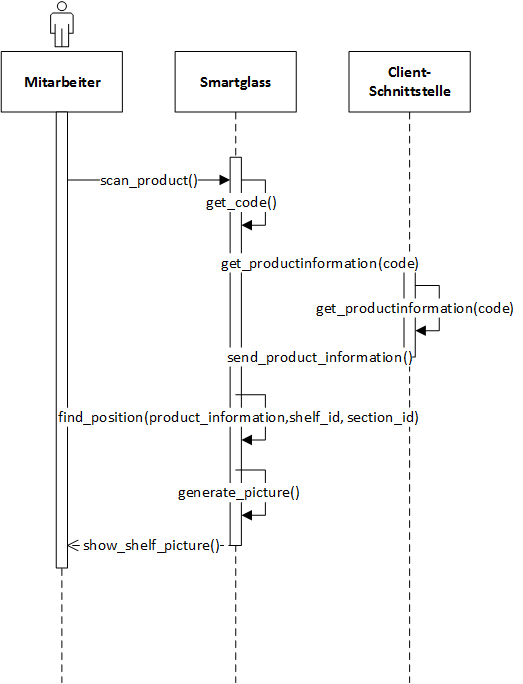
\includegraphics[scale=0.8]{Bilder/Abbildungen/SMAR_produkt_finden_Sequenzdiagramm.png}}
	\caption{Sequenzdiagramm Produkt finden}
	\label{fig:jwt_encode}
\end{figure}
Nachdem der Mitarbeiter die Funktion gestartet hat, vermittelt er der Smartglass den Befehl ein Produkt zu finden, sodass die Smartglass sofort in den Scan-Modus springt (scan\_product()). Dabei hat der Mitarbeiter die Intention, dass die Smartglass ihm dabei Hilft den Regalplatz zu finden.

Sofern der Artikel gescannt wurde, berechnet die Smartglass aus dem Bild den entsprechenden Code (get\_code()). Dies geschieht mit der ZingLibrary. Nachdem die Smartglass den Code errechnet hat, verschickt sie diesen Code an den Datenbankserver, der sich im gleichen Netzwerk befindet, damit dieser mit Produktinformationen antwortet. Mithilfe des Codes sucht die Datenbank intern zuerst nach dem entsprechenden Produkt. Anschließend werden über das Produkt folgende Informationen zurück an die Smartglass geschickt:
\begin{itemize}
	\item Der Name zur ergonomischen und leichten Handhabung für den Mitarbeiter.
	\item Die Füllstände von dem Artikel auf der Verkaufsfläche und im  Lager.
	\item Die aktuell ausgewählte Unit (Karton, Einzelstück).
	\item Das zugehörige Shelf als auch die entsprechende Section.
\end{itemize}
Der Name sowie die Füllstände im Lager und im Verkauf werden dem Nutzer angezeigt.

Mithilfe der Produktinformation, um welches Produkt es sich handelt, und der hinterlegten Karte aller Produktplätze generiert die Smartglass ein Bild – genauer eine SVG Grafik (generate\_picture()). Die Smartglass hat intern eine Karte mit den Attributen Shelf und Section. Dies sind Unterteilungen der Grafik in entsprechende Bereiche. Die Brille weiß allerdings nicht, welches Produkt in welchem Shelf, Section Paar liegt. Mithilfe der Datenbank erfährt sie diese Informationen und kann mit der lokal gespeicherten Karte, das Bild erzeugen. Dieses Bild zeigt einen Ausschnitt des Regalplatzes und markiert den Bereich, in dem das Produkt einzuräumen ist. Dieses Bild wird dem Mitarbeiter anschließend angezeigt. (send\_shelf\_picture()).

Da in den meisten Fällen nach der Produktplatz suche, das jeweilige Produkt eingeräumt werden soll, fragt die Brille den Mitarbeiter, ob er dies tun möchte.
Bestätigt er, springt sozusagen der Instruction Pointer in den Prozess „Produkt einräumen“. Dort wird allerdings der Scan-Vorgang übersprungen und öffnet den Dialog mit schon getroffenen Produktinformationen. 
Verneint der Nutzer, so springt die Smartglass zurück an den Anfang vom „Produkt finden“ Prozess. 

\subsection{Produkt einräumen}
Dieser Abschnitt gibt Implementierungsdetails sowie architektonische Einblicke in die Umsetzung des Prozesses „Produkt einräumen“. Dabei soll die Umsetzung chronologisch beschrieben werden mit zur Hilfenahme des folgenden Sequenzdiagramms. Vorausgesetzt ist, dass der Mitarbeiter schon die Funktion „Produkt einräumen“ ausgewählt hat. 
\begin{figure}[H]
	\centering
	{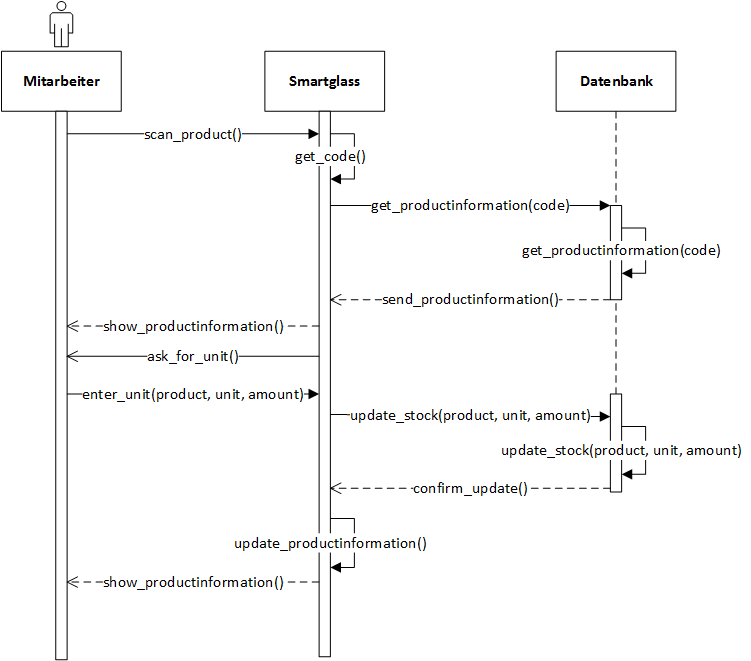
\includegraphics[scale=0.7]{Bilder/Abbildungen/SMAR_produkt_einraeumen_Sequenzdiagramm.png}}
	\caption{Sequenzdiagramm Produkt einräumen}
	\label{fig:jwt_encode}
\end{figure}
Ähnlich dem Prozess, Produkt finden, gibt es drei Aktoren, den Mitarbeiter, die Smartglass und die Datenbank, und startet, indem der Nutzer den \glqq Produkt einräumen\grqq -Prozess gestartet hat (scan\_product()). Daraufhin startet die Smartglass den Barcodescanner und berechnet aus dem erfassten Bild einen Code (get\_code()). Dieser Code wird an die Datenbank verschickt mit der Aufforderung produktspezifische Informationen anzugeben (get\_productinformation()). Die Datenbank sucht diese Informationen raus und antwortet der Smartglass mit diesen (send\_productinformation()). Bei diesen Informationen handelt es sich um folgende: 
\begin{enumerate}
	\item Der Name zur ergonomischen und leichten Handhabung für den Mitarbeiter.
	\item Die Füllstände von dem Artikel auf der Verkaufsfläche und im  Lager.
	\item Die aktuell gescannte Unit (Karton, Einzelstück).
\end{enumerate}
Die gescannte Unit ist dabei der Barcode an einem Karton oder einem einzelnen Produkt. So kann die einzuräumende Unit, und damit Menge, vorselektiert werden. 

Diese Informationen werden dem Mitarbeiter auf dem Display angezeigt. Dies ist auch der Punkt an dem der Prozess \glqq Produkt finden\grqq , in diesen Prozess springt.

So muss der Mitarbeiter weniger mit der Smartglass interagieren. Er hat allerdings noch die Möglichkeit die Unit entsprechend anzupassen (ask\_for\_unit() und enter\_unit()). Dabei hat der Mitarbeiter auch die Möglichkeit nicht nur die Unit anzugeben (ob Karton oder Einzelstück), sondern direkt die Möglichkeit eine Anzahl anzugeben (\zB 4 Kartons). Damit soll die mehrfache Interaktion vermieden werden. 

Schließlich bestätigt der Mitarbeiter (enter\_unit()) und die Smartglass leitet die neuen Informationen an die Datenbank weiter (update\_stock()). So werden dort die Füllstände für das Lager und auf der Verkaufsfläche entsprechend angepasst (update\_stock()).

Die Datenbank bestätigt dies (confirm\_update()), die Smartglass aktualisiert die Informationen, die dem Nutzer angezeigt werden (die Füllstände) (show\_productinformation()), und springt schließlich zurück zum Anfang des Prozesses. 



\subsection{Warenannahme}
Dieser Abschnitt beschreibt den Interaktionsprozess zwischen dem Mitarbeiter, der Smartglass und der Datenbank. Wie in den vorherigen Abschnitten wird ein Sequenzdiagramm zur Illustrierung verwendet. Voraussetzung für diesen Prozess ist, dass der Mitarbeiter den Prozess "Warenannahme" im Hauptmenü ausgewählt hat. 
\\
Ist dies geschehen öffnet die Smartglass den Scanmodus und erwartet vom Mitarbeiter, dass dieser den Lieferschein einscannt. Der Lieferschein ist deshalb wichtig, damit die folgenden Waren, die angenommen werden, der korrekten Lieferung zugeordnet werden können (scan\_delivery\_note()). 
\\
Wurde der Code eingescannt, wird intern der Code berechnet und ein Request an die Datenbank geschickt (get\_delivery\_information()). Dabei wird der gescannte Code mitgeschickt. Die Datenbank überprüft den Code und sucht die erwartenden Produkte und Mengen heraus (get\_delivery\_information()). Diese sendet die Datenbank als Response zurück an die Smartglass (send\_information()), welche diese dem Mitarbeiter anzeigt (show\_delivery\_information()).
\\
Wie in der Schleife zu sehen, wiederholt sich der folgende Vorgang solang bis entweder der Lieferschein abgearbeitet ist oder der Mitarbeiter diesen unterbricht. Bis dahin Scannt der Mitarbeiter jeden Artikel bzw. Karton (scan\_product()). Daraufhin berechnet die Smartglass den Code, verschickt diesen an die Datenbank, sodass diese den Lagerbestand entsprechend anpasst. Sofern die Datenbank aus dem Code das Produkt zugeordnet hat (get\_product()), wird der Wert entsprechend aktualisiert (update\_stock()). Anschließend werden Bestätigungen bis runter zum Mitarbeiter verschickt und angezeigt.
\\
Hat der Mitarbeiter den Lieferschein abgearbeitet, wird eine kurze Erfolgsmeldung angezeigt, damit der Mitarbeiter eine Rückmeldung bekommt (success\_delivery\_scan()).

\begin{figure}[H]
	\centering
	{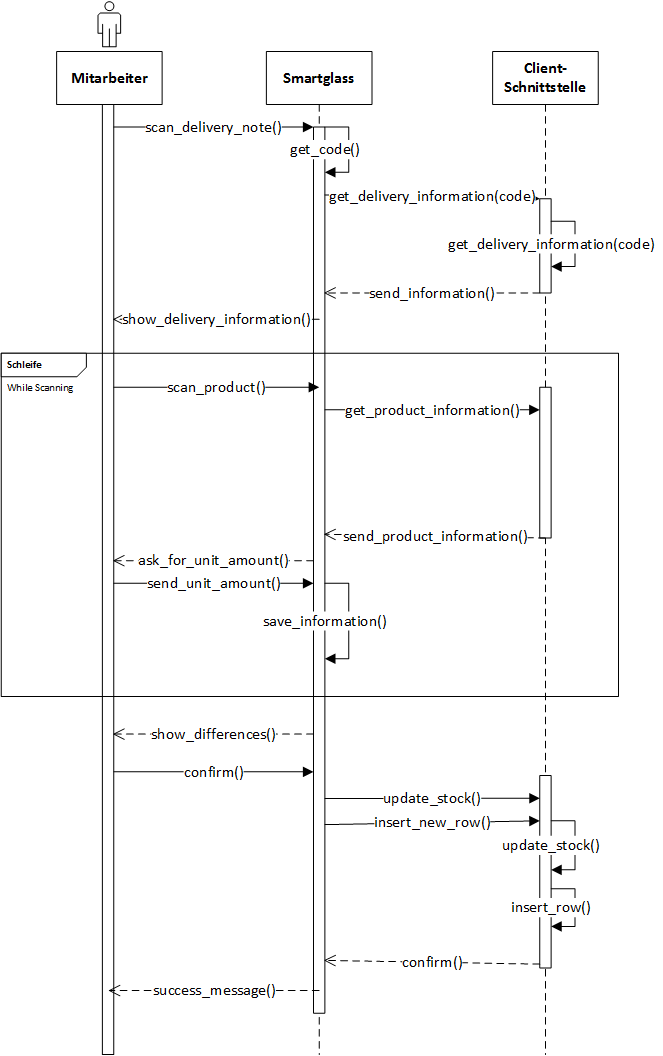
\includegraphics[scale=1.0]{Bilder/Abbildungen/SMAR_warenannahme_Sequenzdiagramm.png}}
	\caption{Sequenzdiagramm Produkt einräumen}
	\label{fig:sequenz_warenannnahme}
\end{figure}

\section{HTTP Nutzung}
\label{sec:httpnutzung}
Dieser Abschnitt befasst sich nicht mit einem konkreten Prozess, sondern erklärt das allgemeine vorgehen und die Akteure bei einem der vielen REST API Aufrufe. Voraussetzungen für eine einwandfrei Nutzung der REST API sind zwei Pakete auf der Smartglass notwendig. Diese sind standardmäßig ausgeliefert und müssen somit nicht manuell nachinstalliert werden.
\begin{enumerate}
	\item org.apache.http
	\item org.json.JSONObject
\end{enumerate}
Das erste Paket stellt die Hauptklassen und -methoden zur Nutzung von HTTP Komponenten. Diese sind essentiell, um das HTTP Protokoll zu verwenden. Es stellt zum Beispiel über HTTP die Verbindung auf und bietet die Möglichkeiten Requests zu versenden und Responses entgegen zu nehmen.\footnote{\citep{http}} Grundsätzlich ist zu sagen, dass hier nur eine schematische und vereinfachte Erklärung gewählt ist. 
\\
Das zweite Paket bietet Möglichkeiten JSON Objekte zu erstellen und mit diesen zu arbeiten. \footnote{\citep{json}}
\\
Das folgende Klassendiagramm visualisiert die nötigen Klassen, um einen HTTP Request zu schicken, eine Antwort zu erhalten und schließlich die Informationen davon, zu verwenden.
\begin{figure}[H]
	\centering
	{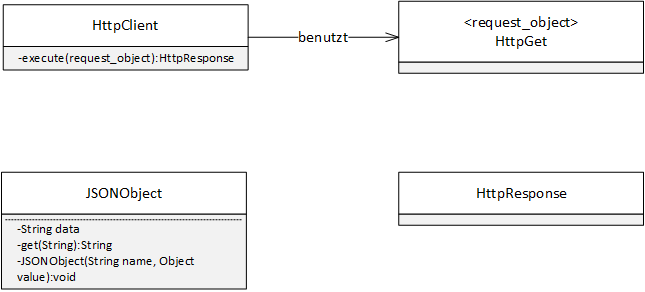
\includegraphics[scale=0.7]{Bilder/Abbildungen/http_request_klassendiagramm.png}}
	\caption{HTTP Request Klassendiagramm}
	\label{fig:sequenz_warenannnahme}
\end{figure}
Zu Beginn wird ein Objekt der Klasse \glqq HttpClient\grqq erzeugt. Der HttpClient kann ein sogenanntes \glqq request\_object\grqq verwenden. In der Grafik ist es konkret ein \glqq HttpGet\grqq -Objekt, das erzeugt wird. Grundsätzlich sind aber auch HttpPost, HttpDelete und HttpPut, nur um die wichtigsten HTTP Verben zu nennen, möglich. In einer Instanz der Klasse HttpGet wird eine URL zugewiesen, und anschließend benutzt das Objekt HttpClient, mithilfe der \glqq execute\grqq -Methode, das request\_object.
\\
Wird dieser Befehl ausgeführt, so wird ein Http-Request an den Server geschickt. Dieser antwortet mit einem einfach HttpResponse, bestehend aus Header und Body. Sofern der Request korrekt und ohne Fehler durchlaufen ist, ist der Body des Response nicht leer. Somit kann er mithilfe eines Objekts der Klasse HttpResponse angenommen werden. Prinzipiell ist darin ein String enthalten. 
\\
Wie in einem vorherigen Kapitel schon angesprochen, sind die HttpResponses in diesem konkreten Projekt in JSON Syntax geschrieben. Deshalb ist der String im \glqq HttpResponse\grqq Objekt in JSON Syntax, sodass sich dieser leicht verwerten sollte. Dies ist mithilfe eines JSON Objekts einfach. Dazu wird die Methode bzw. auch der Konstruktor mit dem entsprechendem String gefüllt. Die Umwandlung des String in einzelne Attribute übernimmt das Objekt selbst. Mithilfe der Methode \glqq get(String)\grqq können einzelne Attribute herausgezogen werden, indem als \glqq String\grqq der Name des Attributes angegeben wird.
\\
Somit lassen sich die vielen Http-Aufrufe, also die Interaktion mit den hinterlegten REST Services, sehr einfach und elegant nutzen und verarbeiten.

\section{Settings}
\label{sec:settings}
Dieser Abschnitt beschreibt und erklärt die Umsetzung des Speicherungsmechanismus auf der Smartglass. Hierzu wird die Klasse \glqq PreferencesHelper.java\grqq erläutert. 
\\
Prinzipiell werden in einer Applikation unter einer Android-Umgebung Informationen in einem sogenannten SharedPreferences-Pool gespeichert. Diese sind einer Aktivität zugeordnet, haben einen Namen und einen Wert. Dazu wird der Pool der aktuellen Aktivität geladen und über einen Editor editierbar gemacht. So können Einstellungen verändert werden. 
\\
Ähnlich ist das Abrufen von Einstellungen. Dazu wird ebenfalls über die aktuelle Aktivität der \glqq SharedPreferences\grqq aufgerufen, und darin der Name der Einstellung herausgesucht. Anschließend erhält man den Wert der Einstellung. 
\\
Es wurde sich dafür entschieden die oben erwähnte Klasse zu implementieren, um eine Abstraktionsschicht für jegliche Zugriffe auf Einstellungen zu gewährleisten. So laufen alle Zugriffe gleich ab, und bei Änderungen oder Erweiterungen gibt es einen zentralen Ort. Dennoch sind alle nutzenden Klassen von Veränderungen betroffen. 
\\
Konkret sind Standardmaßnahmen für den Lesenden sowie Schreibenden Zugriff auf Einstellung mit den Parameter String als auch Integer. Diese scharfe Trennung muss auch erfolgen, da der Editor nur genaue Typen akzeptiert. 
\\
\section{Barcode Erkennung}
\label{sec:barcode}
Dieses Kapitel beschäftigt sich mit der Implementation der Barcode Scanner-Funktion in die \ac{SMAR} Anwendung auf der Smartglass. Wie im Kapitel \ref{cha:technik} \nameref{cha:technik} bereits beschrieben, wurde sich gegen die Anschaffung eines externen Barcode Scanners entschieden, sodass die Erkennung von Bar- und QR-Codes durch eine Library in Verbindung mit der eingebauten Kamera übernommen wird.\\

Android \bzw Google bieten keine Library für das Erkennen von Bar-/QR-Codes an. Außerdem würde es den Rahmen dieses Projektes übersteigen eigene Klassen für diese Aufgabe zu entwickeln. Eine Recherche ergab folgende zwei populäre und ausgereifte externe Anwendungen \bzw Librarys, die frei zur Verfügung stehen:
\begin{itemize}
	\item zebra crossing (ZXing)
	\item ZBar SDK
\end{itemize}
Bei ZXing handelt es sich in erster Linie um eine Barcode Scanner App für Android. Darüber hinaus unterstützt die App jedoch den externen Zugriff durch eine andere App und kann das Ergebnis des Scans an die externe App weitergeben. Das \ac{SMAR}-Projekt würde die Barcode Scanner App von ZXing entsprechend jedes mal starten, sobald ein neuer Code benötigt wird und die Antwort der Barcode Scanner App abwarten.\\
Ein großer Vorteil ist die schnelle und einfache Integration, die anhand weniger Zeilen Sourcecode geschieht. Entscheidende Nachteile sind jedoch die Abhängigkeit von einer anderen App, die auf dem Gerät ebenfalls installiert sein muss und der erhöhte Ressourcenverbrauch, der das\ac{SMAR}-Projekt in der Effizienz einschränken könnte. Da der Sourcecode der Barcode Scanner App frei verfügbar ist, wäre die Möglichkeit der Integration der gesamten Anwendung. Dies ist aufgrund der Komplexität aber ebenfalls nicht praktikabel.\\

Die Entscheidung fiel daher auf die ZBar SDK Library. Diese wird in das Projekt als externe Library integriert und bietet die Möglichkeit Bilder auf einen Bar- oder QR-Code zu untersuchen. Ein Nachteil ist der erhöhte Programmieraufwand, der für das Erstellen der Kamera Vorschau und der Aufruflogik benötigt wird. Der entscheidende Vorteil ist jedoch, dass alle Aktionen innerhalb der \ac{SMAR}-Anwendung stattfinden und keine externen Anwendungen zur Laufzeit benötigt werden.\\

Die ZBar Library unterstützt alle gängigen Barcode- und QR-Code Typen und ist damit optimal für den Einsatz in diesem Projekt geeignet:\footnote{\citep{zbar}}
\begin{itemize}
	\item EAN/UPC: EAN-8, EAN-13, UPC-A, UPC-E
	\item Linear: Code 39, Code 93, Code 128, Interleaved 2 of 5, DataBar
	\item 2-D: QR-Code
\end{itemize}

Für die Integration der ZBar Library werden zwei neue Klassen benötigt:
\begin{enumerate}
	\item Eine Activity (eine neue Seite), im folgenden Barcode-Klasse genannt.
	\item Eine Klasse, die die Kamera Vorschau innerhalb eines Fensters erstellt, das in eine Activity eingebunden werden kann. Im folgenden Kamera-Klasse genannt.
\end{enumerate} 
Wird das Einscannen eines Barcodes benötigt, so wird die Barcode-Klasse aufgerufen. Diese erstellt eine neue Instanz der ZBar Lybrary mit entsprechend eingestellter Konfiguration (wie \zB Auflösungseinstellungen, zu erkennende Codes) und fragt beim Android Betriebssystem nach der Öffnung einer Kamerainstanz. Wird eine gültige Kamerainstanz zurückgeliefert, so wird die Kamera-Klasse mit dieser Instanz ausgeführt und das Vorschaubild in die Activity integriert. Außerdem stellt die Barcode-Klasse Methoden zur Verfügung, die bei Rückgabe von Werten seitens der Kamera-Klasse, ausgeführt wird. Dies sind die Bilder, die die Kamera aufzeichnet, die anschließend an die Instanz der ZBar Library weitergeleitet werden. Liefert die ZBar Library ein Ergebnis zurück, wird die Kamera-Klasse und die Kamerainstanz geschlossen, sowie die Activity geschlossen und die Barcode-Klasse gibt das Ergebnis zurück. Dieses Ergebnis kann durch die Klasse, die die Barcode-Klasse ausgeführt hat, über eine onActivityResult()-Methode abgerufen werden.\\

Die Kamera-Klasse konfiguriert bei Ausführung zunächst die Kamera (Ausrichtung der Kamera, Bildwiederholrate, Autofokus, ...) und definiert den Callback. Der Callback wird ausgeführt, sobald die Kamera ein Bild aufgenommen hat. Als Daten werden dabei die Bildinformationen übergeben, die von der Barcode-Klasse abgerufen werden.

\section{Rechteverwaltung}
\label{cha:rechteverwaltung_vr}



\subsection{\acf{AuthN}}
Das folgende Kapitel beschäftigt sich mit der Authentifizierung in der App gegenüber dem Server. Benutzte Bibliotheken und Eingabemethoden werden erklärt. Darüber hinaus wird die verwendete Methode mit anderen technisch möglichen Eingabemethoden verglichen.\\

\acl{AuthN} dient der Identifikation einer Person/eines Gerätes.

\subsubsection{\acs{AuthN} gegenüber der Brille}
Die App auf der eingesetzten Vuzix M100 Virtual Reality Brille wird, wie beschrieben, zur Warenannahme, sowie zum Einräumen von Produkten verwendet - mit der Brille kann der Warenbestand daher aktiv verändert und manipuliert werden.\\
Diese Veränderung sollte, um \zB strukturierten Diebstahl zu vermeiden, nur durch Authentifizierte \acs{AuthN} und Autorisierte \acs{AuthZ} Personen durchgeführt werden.\\

Die gängige Ein-Faktor-Authentifizierung besteht aus der Kombination eines Benutzernamens mit einem Passwort. Dieses Verfahren hat sich bewährt und bietet bei korrekter Implementation eine durchschnittliche Sicherheit vor unbefugtem Zugriff. Diese Sicherheit würde im Rahmen dieser Anwendung ausreichen, da der Angreifer neben den Benutzerdaten, ebenfalls Zugriff auf ein Gerät haben muss, welches:
\begin{itemize}
	\item in das Firmennetzwerk eingebunden ist und
	\item gegenüber dem Server authentifiziert\footnote{s. Kapitel \ref{cha:authn_server}\nameref{cha:authn_server}} ist.
\end{itemize}
Eine Zwei-Faktor-Authentifizierung ist somit bereits gegeben, da der Benutzer sowohl Wissen (Benutzername und Passwort) als auch Besitz benötigt (Die authentifizierte \acl{VR}-Brille).\\
Die Grundlage für eine gute Anwendungssicherheit ist somit gegeben.

Die Brille hat, wie im Kapitel \ref{cha:brille}\nameref{cha:brille} beschrieben, folgende Eingabemethoden:
\begin{itemize}
	\item 4 Knöpfe an der Brille zur Navigation durch das Betriebssystem
	\item Sensoren zur Erkennung von Gesten
	\item Mikrofon zur Erkennung von Sprachbefehlen
	\item Kamera mit entsprechenden Bibliotheken zur Erkennung von Bar- und QR-Codes
\end{itemize}
Die, für die oben beschriebene \acf{AuthN} übliche Eingabemethode, die textbasierte Eingabe über eine entsprechende Tastatur ist über die \ac{VR}-Brille ohne zusätzliche Hardware nicht möglich. Zusätzliche Hardware wäre zu dem umständlich und würde die Bedienung des Gerätes erschweren. Die Usability ist bei dieser Eingabemethode nicht gegeben.\\

Die Eingabe der Anmeldedaten muss daher über andere Eingabemethoden stattfinden und wird in 2 Teile unterteilt:
\begin{enumerate}
	\item Eingabe/Auswahl des Benutzernamens
	\item Eingabe des Passworts
\end{enumerate}

Der Benutzername ist - im Gegensatz - zum Passwort zumindest gegenüber den anderen Mitarbeitern, die Zugriff auf die Brille haben, kein Geheimnis und kann Bekannt sein.\\
Die Eingabe des Benutzernamens über ein Sprachkommando gestaltet sich schwierig und als nicht effektiv. Im Rahmen dieser Arbeit wurde ein Test (TODO: Kapitelrefernzierung auf Kapitel mit Test der Spracherkennung) durchgeführt, der die Spracherkennung testete. Dies funktionierte bei vordefinierten Sprachbefehlen und bei wenig Störgeräuschen zufriedenstellend. Für die Eingabe von Benutzernamen ist dies jedoch nicht geeignet, da die Anmeldung sowohl in ruhigen Umgebungen, als auch lauten Filialen schnell funktionieren muss. Darüber hinaus kann die Erkennung von Eigennamen, die eventuell durch verschiedene Sprachen geprägt sind, nicht zuverlässig garantiert werden.\\
Die Entscheidung fiel daher auf eine Liste, die beim Starten der App vom Server abgerufen wird und auf der LogIn-Seite der App angezeigt wird. Der Server liefert eine Liste mit Benutzern zurück, die für die Brille zugelassen sind (TODO: Kapitelreferenzierung - Rechte). Der Benutzer wählt über die Knöpfe an der Brille den Benutzernamen aus der Liste aus und wird anschließend zur Eingabe des gültigen Passworts aufgefordert.\\
Dies garantiert eine, nach den Möglichkeiten der Vuzix M100 gegebenen, zuverlässige und schnelle Anmeldung. Diese Anmeldemethode ist verständlicherweise nur für eine geringe Anzahl an Benutzern (<30) effizient, jedoch wird davon ausgegangen, dass in einem Supermarkt in der Regel nicht mehr als 20 bis 30 Angestellte mit der Warenannahme/-einräumung beauftragt werden.\\

Auch bei der Passworteingabe gibt es ähnliche Probleme, jedoch muss hier darauf geachtet werden, dass Passwörter ausschließlich dem jeweiligen Benutzer (und eventuell dem Systemadministrator) bekannt sein dürfen \bzw nur im Besitz des Benutzers liegen dürfen. Eine Auswahl aus einer Liste und die Eingabe per Spracherkennung sind somit nicht nur aus Sicht der Bedienung, sondern vor Allem aus Sicherheitsgründen nicht praktikabel.\\
Ein Passwort, das auf Gesten basiert, ist aufgrund der geringen Anzahl an Variationen und möglichen Kombinationen ebenfalls nicht sicher.\\
Die Passworteingabe muss daher über die vierte Eingabemöglichkeit getätigt werden: die Eingabe über Barcodes/QR-Codes mit Hilfe der Kamera.\\

Sobald der Benutzer seinen Benutzernamen aus der Liste ausgewählt hat, wird die Kamera, sowie eine Bibliothek zur Erkennung von QR-Codes gestartet. Der Benutzer scannt seinen persönlichen QR-Code, der in einen String mit einer Länge von 64 Zeichen umgewandelt wird. Diese Daten werden an den Server weitergeleitet, der die Anmeldung schließlich bestätigt (bei korrekter Kombination) oder widerruft (bei ungültigen Login-Daten). Bei korrekter Authentifizierung, gibt der Server einen \ac{JWT} zurück, welcher bei einer Anfrage an den Server mitgeschickt werden muss und auf Korrektheit überprüft wird. Bei einem widerrufenen Login erhält die App ausschließlich eine Fehlermeldung, weitere Anfragen werden aufgrund des fehlenden \ac{JWT} nicht ausgeführt.\\

Der QR-Code kann mit Hilfe der Weboberfläche generiert werden oder es kann ein bestehender Code aktiviert werden (TODO: Kapitelreferenz SMAR Web Administration). Der QR-Code kann durch den Benutzer aufbewahrt werden, sollte der Code in unbefugte Hände gelangen, kann ein neuer Code generiert werden. Außerdem ist es möglich vorhandene Codes, wie \zB ein Code auf der persönlichen Firmen-Zugangskarte des Benutzers, zu verwenden.\\

Die benötigte Sicherheit und das Effiziente Anmelden an die Anwendung ist mit dieser Lösung gewährleistet.

\subsubsection{\acs{AuthN} gegenüber dem Server}
\label{cha:authn_server}
Im letzten Kapitel wurde beschrieben, wie sichergestellt wird, dass sich nur bekannte und authorisierte Benutzer anmelden können. Das dies nicht unbedingt ausreichend ist, verdeutlicht das folgende Szenario:
\begin{itemize}
	\item Ein Angestellter einer Filiale, der mit der Warenannahme beauftragt ist und somit für die Nutzung der Brille freigeschaltet ist, lässt seinen Firmenausweis beim Einräumen in einem öffentlichen Bereich liegen. Auf dem Firmenausweis sind sowohl der vollständige Name, als auch der QR-Code, der für die Authentifizierung genutzt wird, aufgedruckt. Ein Angreifer, der Zugriff auf das System bekommen möchte, entdeckt dies und fotografiert den Firmenausweis ab.
\end{itemize}
Im oben dargestellten Szenario sind die persönlichen Benutzerdaten - ohne Wissen des Opfers - gestohlen worden. Der Angreifer hat zwar keinen Zugriff auf eine im Markt vorhandene \ac{VR}-Brille, aber eventuell ist er im Besitz der App und hat diese auf einem eigenen Android-Gerät installiert. Ist das Firmennetzwerk zusätzlich noch schlecht abgesichert, \zB durch Nutzung des \ac{WEP} Verschlüsselungsprotokolls, so kann sich der Angreifer mit seinem eigenen Android-Gerät und über die Anmeldedaten des Angestellten auf dem Server authentifizieren.\\
Er kann den Warenbestand nun entsprechend manipulieren und der Filiale schaden zufügen.\\

Um dies zu verhindern, wurde eine Zwei-Faktor-Authentifizierung in die Anwendung integriert. Somit muss sich nicht nur der Benutzer, sondern ebenfalls die \ac{VR}-Brille \bzw das benutzte Gerät gegenüber dem Server authentifizieren.\\

Die App liest dazu beim Starten der Anwendung die \ac{MAC}-Adresse des Gerätes aus und speichert diese in der für den Login zuständigen Klasse ab. Sobald sich der Benutzer anmeldet (seinen Benutzernamen ausgewählt hat und den persönlichen QR-Code eingescannt hat), wird die \ac{MAC}-Adresse an die Login-Daten angehängt und eine Anfrage (Ausführen der "authenticate"-Anwendung der REST Api\footnote{s. Kapitel TODO: Kapitelreferenz auf REST Api-Erklärung}) an den Server mit allen Daten (\ac{MAC}-Adresse, Benutzer, Passwort) geschickt. Ist die \ac{MAC}-Adresse gültig, liefert der Server den \ac{JWT}, ansonsten gibt es eine Fehlermeldungen und alle weiteren Anfragen werden abgelehnt.\\

Eine \ac{MAC}-Adresse und somit das dazugehörige Gerät werden durch einen Eintrag in der Datenbank registriert. Für jedes Gerät wird ein Name, sowie die \ac{MAC}-Adresse vergeben und ein Flag gesetzt, ob dieses Gerät aktuell aktiv sein soll. Das registrierte Gerät kann sich somit gegenüber dem Server erfolgreich identifizieren.

\subsection{\acf{AuthZ}}
Die \acl{AuthZ} beschreibt - im Gegensatz zur \acl{AuthN} - nicht die Identifikation einer Person/eines Gerätes, sondern prüft die Berechtigungen der bereits vorhandenen Identifikation. Für eine \acl{AuthZ} ist daher eine bereits erfolgreiche \acl{AuthN} erforderlich.

Bei der Benutzung der App gibt es sowohl für das Gerät, als auch für den Benutzer ausschließlich 2 Berechtigungsstufen:
\begin{itemize}
	\item Benutzer/Gerät hat die Berechtigung Daten zu lesen/bearbeiten/löschen,
	\item Benutzer/Gerät hat keine Berechtigung auf die Daten zuzugreifen.
\end{itemize}

Die \acl{AuthZ} findet daher zeitgleich zu der \acl{AuthN} statt. Der \ac{JWT} wird ausschließlich bei erfolgreicher Identifikation und Berechtigung zurückgegeben, ansonsten gibt es eine entsprechende Fehlermeldung.\\

Das Gerät autorisiert sich gegenüber dem Server über das Flag, welches bestimmt, ob das Gerät aktuell aktiv sein soll. Ist dieses Flag gesetzt, besitzt dieses Gerät (\zB \acs{VR}-Brille) volle Berechtigung und weitere Anfragen werden bei gültigem \ac{JWT} übergeben, ansonsten werden alle weiteren Anfragen abgelehnt. Diese \acl{AuthZ} macht Sinn, sollte das Gerät kurzfristig nicht in der Filiale sein. Das Gerät kann gesperrt und reaktiviert werden, ohne dass es gelöscht und anschließend wieder registriert werden muss.\\

Da ein Benutzer ebenfalls nur diese zwei Berechtigungsstufen beim Benutzen der App besitzt, wird die Anfrage ähnlich der Brille ausgeführt. Ein Benutzer besitzt in seinem Datenbank-Eintrag in der Spalte \glqq role\_device\grqq~~ entweder eine 1 (true) und wird autorisiert oder eine 0 (false) und der Server meldet einen entsprechenden Fehler zurück.\\

Weitere Berechtigungsstufen werden an dieser Stelle nicht benötigt, da ein Angestellter, der mit der Warenannahme oder -einräumung beauftragt ist, die gesamte App-Funktionalität benutzt und ein Angestellter, der keine der beiden Aufgaben benötigt, keinen Zugriff auf die Brille benötigt.